\documentclass[12pt,a4paper]{article}
\usepackage[utf8]{vietnam}
\usepackage{amsmath,amssymb,amsfonts,amsthm}
\usepackage{graphicx}
\usepackage{tabularray}
\usepackage{tabularx}
\usepackage{tikz}
\usetikzlibrary{calc}
\usepackage[left=2.5cm,right=2cm,top=2.5cm,bottom=2.5cm]{geometry}
\usepackage{fancyhdr}
\setlength{\headheight}{15.2807pt}
\usepackage{xcolor}
\usepackage{array}
\usepackage{titlesec}
\usepackage{hyperref}
\usepackage{float}
\usepackage{caption}
\usepackage{subcaption}
\usepackage{booktabs}
\usepackage{enumitem}
\usepackage{indentfirst}
\captionsetup[figure]{justification=centering}

\usepackage{minted}
\setminted{style=friendly}

% ===== Code block style (tcolorbox + minted) =====
\usepackage{tcolorbox}
\tcbuselibrary{minted,breakable,xparse,skins}

\definecolor{bg}{gray}{0.95}
\DeclareTCBListing{mintedbox}{O{}m!O{}}{%
  breakable=true,
  listing engine=minted,
  listing only,
  minted language=#2,
  minted style=friendly,
  minted options={%
    linenos,
    gobble=0,
    breaklines=true,
    breakafter=,,
    fontsize=\small,
    numbersep=8pt,
    #1},
  boxsep=0pt,
  left skip=0pt,
  right skip=0pt,
  left=25pt,
  right=0pt,
  top=3pt,
  bottom=3pt,
  arc=5pt,
  leftrule=0pt,
  rightrule=0pt,
  bottomrule=2pt,
  toprule=2pt,
  colback=bg,
  colframe=orange!70,
  enhanced,
  overlay={%
    \begin{tcbclipinterior}
    \fill[orange!20!white] (frame.south west) rectangle ([xshift=20pt]frame.north west);
    \end{tcbclipinterior}},
  #3}

% ===== Hyperlink =====
\hypersetup{
    colorlinks=true,
    linkcolor=blue!70!black,
    filecolor=magenta,
    urlcolor=cyan,
    citecolor=red!70!black
}

% ===== Header / Footer =====
\pagestyle{fancy}
\fancyhf{}
\lhead{\textbf{Báo cáo BTVN 7 -- Vật lý tính toán}}
\rhead{\textit{Truyền nhiệt 1D -- FTCS \& BTCS}}
\cfoot{\thepage}
\renewcommand{\headrulewidth}{0.4pt}
\renewcommand{\footrulewidth}{0.4pt}

% ===== Section formatting =====
\titleformat{\section}{\Large\bfseries\color{blue!80!black}}{\thesection.}{0.5em}{}
\titleformat{\subsection}{\large\bfseries\color{blue!70!black}}{\thesubsection.}{0.5em}{}
\titleformat{\subsubsection}{\normalsize\bfseries\color{blue!60!black}}{\thesubsubsection.}{0.5em}{}

\begin{document}

% ================= TRANG BÌA =================
\begin{titlepage}
    \centering
    \vspace*{2cm}

    \rule{\textwidth}{1pt} \\[0.5cm]
    {\huge \textbf{BÁO CÁO BÀI TẬP VỀ NHÀ 7}} \\[0.4cm]
    {\large \textbf{GIẢI PHƯƠNG TRÌNH TRUYỀN NHIỆT 1D BẰNG}} \\[0.2cm]
    {\large \textbf{PHƯƠNG PHÁP HIỆN (FTCS) VÀ PHƯƠNG PHÁP ẨN (BTCS)}} \\[0.2cm]
    \rule{\textwidth}{1pt}

    \vspace{2cm}

    {\large
    \begin{tabular}{rl}
        \textbf{Họ và tên:}  & Nguyễn Trần Gia Bảo \\[4pt]
        \textbf{MSSV:}       & 23137003 \\[4pt]
        \textbf{Môn học:}    & Vật lý tính toán (PHY10532) \\[4pt]
        \textbf{Giảng viên:} & TS.\@ Vũ Quang Tuyên \\
    \end{tabular}
    }

    \vfill
    {\large \today}
\end{titlepage}

% ================= MỤC LỤC =================
\newpage
\tableofcontents
\newpage

% =============================================================
\section{Giới thiệu và nội dung bài tập}
% =============================================================

Phương trình truyền nhiệt là một trong những phương trình đạo hàm riêng quan trọng nhất trong vật lý -- nó không chỉ mô tả lan truyền nhiệt trong chất rắn mà còn cùng dạng toán học với phương trình khuếch tán hạt (Fick), phương trình Black--Scholes trong tài chính, hay phương trình Schrödinger Wick-rotated. Việc giải số phương trình này bằng sai phân hữu hạn là chủ đề kinh điển và là bước đệm để tiếp cận các bài toán PDE phức tạp hơn.

Bài tập yêu cầu giải phương trình truyền nhiệt một chiều
\begin{equation}
    \alpha^2\,\frac{\partial^2 u}{\partial x^2} = \frac{\partial u}{\partial t}
    \label{eq:heat_intro}
\end{equation}
bằng \textbf{hai phương pháp sai phân} khác nhau về bản chất số học:

\begin{itemize}
    \item \textbf{Phương pháp hiện (Forward-Time Central-Space, FTCS / Explicit):} cập nhật $u_i^{j+1}$ tường minh từ ba giá trị ở bước thời gian trước. Đơn giản nhưng \emph{bị ràng buộc} bởi điều kiện ổn định $\eta \le 1/2$.
    \item \textbf{Phương pháp ẩn (Backward-Time Central-Space, BTCS / Implicit):} cần giải một hệ tuyến tính tridiagonal ở mỗi bước thời gian. Tốn hơn nhưng \emph{unconditionally stable} -- không có ràng buộc $\eta$, cho phép chọn bước thời gian lớn tuỳ ý.
\end{itemize}

Hai bài toán cụ thể được giải trên cả hai phương pháp:

\begin{enumerate}
    \item \textbf{Bài 1 -- Thanh đơn nung nóng:}\\
    Thanh dài $l = 1\,\mathrm{m}$ ban đầu có nhiệt độ $T(x, 0) = 100\,^\circ\mathrm{C}$ đồng đều. Hai đầu thanh được giữ ở $0\,^\circ\mathrm{C}$ trong suốt quá trình. Yêu cầu tính phân bố nhiệt độ $T(x, t)$ trong khoảng $t \in [0, 1800\,\mathrm{s}]$.

    \item \textbf{Bài 2 -- Hai thanh tiếp xúc (Landau 20.3, trang 483--484):}\\
    Hai thanh cùng chiều dài $l_{\text{bar}} = 0.25\,\mathrm{m}$ đặt tiếp xúc tạo thành một thanh tổng $l_{\text{total}} = 0.5\,\mathrm{m}$. Thanh trái ban đầu $100\,\mathrm{K}$, thanh phải $50\,\mathrm{K}$. Hai đầu ngoài cùng được giữ ở $0\,\mathrm{K}$.
\end{enumerate}

Tham số vật liệu (nhôm): độ dẫn nhiệt $\kappa = 210\,\mathrm{W/(m\cdot K)}$, nhiệt dung riêng $C = 900\,\mathrm{J/(kg\cdot K)}$, khối lượng riêng $\rho = 2700\,\mathrm{kg/m^3}$. Suy ra hệ số khuếch tán nhiệt $\alpha^2 = \kappa/(C\rho) \approx 8.64\times 10^{-5}\,\mathrm{m^2/s}$.

% =============================================================
\section{Cơ sở lý thuyết}
% =============================================================

\subsection{Phương trình truyền nhiệt}

Phương trình~\eqref{eq:heat_intro} xuất phát từ hai phương trình nền:
\begin{itemize}
    \item \textbf{Định luật Fourier} cho dòng nhiệt: $\mathbf{q} = -\kappa\,\nabla u$.
    \item \textbf{Định luật bảo toàn năng lượng}: $\rho\,C\,\dfrac{\partial u}{\partial t} = -\nabla\cdot\mathbf{q}$ (khi không có nguồn nội).
\end{itemize}
Ghép lại cho ra phương trình parabolic chuẩn:
\[
    \frac{\partial u}{\partial t} = \alpha^2\,\nabla^2 u, \qquad
    \alpha^2 = \frac{\kappa}{\rho C}.
\]
Đơn vị $\alpha^2$ là $\mathrm{m^2/s}$ -- hệ số khuếch tán nhiệt, cho biết ``nhiệt lan bao xa trong bao lâu''.

\subsection{Rời rạc hoá lưới không--thời gian}

Chia miền thời gian $[0, t_{\max}]$ thành $N_t$ nút đều khoảng cách $k = t_{\max}/(N_t - 1)$, và miền không gian $[0, l]$ thành $N_x$ nút đều khoảng cách $h = l/(N_x - 1)$. Ký hiệu $u_i^j = u(x_i, t_j)$ với $x_i = i\,h$, $t_j = j\,k$. Đặt số Courant--Friedrichs--Lewy:
\begin{equation}
    \eta \equiv \frac{\alpha^2 k}{h^2}.
    \label{eq:eta}
\end{equation}

\subsection{Phương pháp hiện FTCS (Forward-Time Central-Space)}

Sai phân tiến cho đạo hàm thời gian, trung tâm cho đạo hàm không gian:
\[
    \left.\frac{\partial u}{\partial t}\right|_{i,j} \approx \frac{u_i^{j+1} - u_i^j}{k}, \qquad
    \left.\frac{\partial^2 u}{\partial x^2}\right|_{i,j} \approx \frac{u_{i+1}^j - 2u_i^j + u_{i-1}^j}{h^2}.
\]
Thay vào Phương trình~\eqref{eq:heat_intro} và rút $u_i^{j+1}$:
\begin{equation}
    \boxed{\; u_i^{j+1} = (1 - 2\eta)\,u_i^j + \eta\,\bigl(u_{i+1}^j + u_{i-1}^j\bigr) \;}
    \label{eq:FTCS}
\end{equation}

Ở đây $u_i^{j+1}$ được \emph{tường minh} biểu diễn qua ba giá trị đã biết ở bước $j$ -- không cần giải hệ phương trình. Độ chính xác: $O(k) + O(h^2)$.

\subsection{Phương pháp ẩn BTCS (Backward-Time Central-Space)}

Sai phân \emph{lùi} cho đạo hàm thời gian:
\[
    \left.\frac{\partial u}{\partial t}\right|_{i,j} \approx \frac{u_i^j - u_i^{j-1}}{k}, \qquad
    \left.\frac{\partial^2 u}{\partial x^2}\right|_{i,j} \approx \frac{u_{i+1}^j - 2u_i^j + u_{i-1}^j}{h^2}.
\]
Thay vào Phương trình~\eqref{eq:heat_intro}:
\[
    \frac{u_i^j - u_i^{j-1}}{k} = \alpha^2\,\frac{u_{i+1}^j - 2u_i^j + u_{i-1}^j}{h^2}.
\]
Nhân $k$, đưa mọi đại lượng ở bước $j$ về vế trái:
\begin{equation}
    -\eta\,u_{i-1}^j + (1 + 2\eta)\,u_i^j - \eta\,u_{i+1}^j = u_i^{j-1}.
    \label{eq:BTCS_linear}
\end{equation}

Đây là \textbf{hệ tuyến tính tridiagonal} với ma trận hệ số
\[
    A = \begin{pmatrix}
        1+2\eta & -\eta & & & \\
        -\eta & 1+2\eta & -\eta & & \\
        & \ddots & \ddots & \ddots & \\
        & & -\eta & 1+2\eta & -\eta \\
        & & & -\eta & 1+2\eta
    \end{pmatrix},
\]
vế phải là vector $u_i^{j-1}$ của bước trước. Ở mỗi bước thời gian $j$, phải giải hệ này một lần. Có hai cách:
\begin{itemize}
    \item \emph{Trực tiếp:} giải tridiagonal bằng thuật toán Thomas ($O(N_x)$ phép tính).
    \item \emph{Lặp Gauss--Seidel:} chương trình hiện tại dùng phương pháp này. Hội tụ rất nhanh vì $A$ chéo trội nghiêm ngặt: $|1+2\eta| > 2|\eta|$ với mọi $\eta > 0$.
\end{itemize}

Để dùng Gauss--Seidel, rút $u_i^j$ từ Phương trình~\eqref{eq:BTCS_linear}:
\begin{equation}
    \boxed{\; u_i^j = \beta_1\bigl(u_{i-1}^j + u_{i+1}^j\bigr) + \beta_2\,u_i^{j-1} \;}
    \label{eq:BTCS_GS}
\end{equation}
với
\begin{equation}
    \beta_1 = \frac{\eta}{1 + 2\eta}, \qquad
    \beta_2 = \frac{1}{1 + 2\eta}.
    \label{eq:beta}
\end{equation}

Tính chất: $2\beta_1 + \beta_2 = 1$ (tổ hợp là trung bình có trọng số). Khi $\eta \to 0$ (bước thời gian rất nhỏ): $\beta_1 \to 0$, $\beta_2 \to 1$, công thức suy biến về $u_i^j = u_i^{j-1}$ -- đúng với giới hạn $k \to 0$. Khi $\eta \to \infty$ (bước thời gian rất lớn): $\beta_1 \to 1/2$, $\beta_2 \to 0$, công thức trở thành $u_i^j = (u_{i-1}^j + u_{i+1}^j)/2$ -- đúng là phương trình Laplace ở trạng thái dừng.

\subsection{Phân tích ổn định von Neumann}

Giả sử sai số có dạng Fourier $\varepsilon_i^j = \xi^j\,e^{\mathrm{i}\beta x_i}$, thay vào phương trình cho sai số sẽ cho hệ số khuếch đại $\xi(\beta)$. Phương pháp ổn định khi $|\xi| \le 1$ cho mọi mode.

\subsubsection{FTCS: điều kiện CFL}

Thay vào Phương trình~\eqref{eq:FTCS}:
\[
    \xi = 1 - 4\eta\,\sin^2(\beta h/2).
\]
Điều kiện $-1 \le \xi \le 1$ cho mọi $\beta$:
\begin{equation}
    \boxed{\; \eta \le \tfrac{1}{2} \;}
    \label{eq:CFL_explicit}
\end{equation}
Đây là ràng buộc \textbf{có điều kiện} -- nếu vi phạm, các mode có $\sin^2(\beta h/2) \approx 1$ (tức $\beta h \approx \pi$, mode dao động cao tần nhất) sẽ tăng theo cấp số nhân, làm nghiệm bùng nổ.

\subsubsection{BTCS: unconditionally stable}

Thay vào Phương trình~\eqref{eq:BTCS_linear}:
\[
    \xi\,(1 + 4\eta\,\sin^2(\beta h/2)) = 1
    \;\Longrightarrow\;
    \xi = \frac{1}{1 + 4\eta\,\sin^2(\beta h/2)}.
\]
Vì mẫu số $\ge 1$ với mọi $\beta$ và mọi $\eta > 0$, ta luôn có $0 < \xi \le 1$. Do đó:
\begin{equation}
    \boxed{\;\text{BTCS ổn định không điều kiện, với mọi } \eta > 0\;}
    \label{eq:unconditional}
\end{equation}

Đây là lý do BTCS được ưa chuộng khi cần mô phỏng thời gian dài với lưới không gian mịn.

\subsection{Lựa chọn giữa FTCS và BTCS}

\begin{center}
\small
\begin{tabular}{@{}p{4.3cm}p{5.8cm}p{5.2cm}@{}}
\toprule
\textbf{Tiêu chí} & \textbf{FTCS (Explicit)} & \textbf{BTCS (Implicit)} \\
\midrule
Công thức cập nhật & Tường minh, Phương trình~\eqref{eq:FTCS} & Hệ tridiagonal, Phương trình~\eqref{eq:BTCS_linear} \\
Chi phí mỗi bước thời gian & $O(N_x)$ & $O(N_x)$ (Thomas) hoặc $O(N_x \cdot q_{\text{GS}})$ (Gauss--Seidel) \\
Điều kiện ổn định & $\eta \le 1/2$ & Không điều kiện \\
Độ chính xác thời gian & $O(k)$ & $O(k)$ \\
Độ chính xác không gian & $O(h^2)$ & $O(h^2)$ \\
Khi nào dùng tốt nhất & Bước thời gian ngắn, lưới thô, mô phỏng ngắn hạn & Bước thời gian dài, lưới mịn, mô phỏng dài hạn, bài toán stiff \\
\bottomrule
\end{tabular}
\end{center}

\subsection{Điều kiện biên Dirichlet và điều kiện đầu}

Bài toán parabolic cần:
\begin{itemize}
    \item \textbf{Điều kiện đầu}: $u(x, 0) = u_0(x)$.
    \item \textbf{Điều kiện biên}: $u(0, t) = u_L(t)$, $u(l, t) = u_R(t)$ cho mọi $t > 0$.
\end{itemize}

Trong cả hai phương pháp, các nút biên $i = 0$ và $i = N_x - 1$ \emph{không bao giờ được cập nhật} -- chúng được ``khoá'' bởi điều kiện biên.

\textbf{Lưu ý về tính không tương thích tại $t = 0$:} Với Bài 1, điều kiện đầu $u(x, 0) = 100$ với mọi $x \in (0, l)$ mâu thuẫn với điều kiện biên $u(0, t) = 0$. Do đó $u$ không liên tục tại hai góc $(0, 0)$ và $(l, 0)$. Cả hai phương pháp đều làm mượt điểm không liên tục này trong vài bước thời gian đầu.

% =============================================================
\section{Phân tích chương trình}
% =============================================================

Chương trình được viết bằng Python trong hai notebook riêng biệt: \texttt{BTVN7-forward.ipynb} (FTCS) và \texttt{BTVN7-backward.ipynb} (BTCS + Gauss--Seidel).

\subsection{Phương pháp hiện FTCS}

\subsubsection{Hàm thiết lập điều kiện đầu và biên (Bài 1)}

\begin{mintedbox}{python}
def dieukienbien(N_time, N_x, x_t0, t_x0, t_xl):
    u = np.zeros((N_x, N_time), dtype=float)

    for i in range(N_time):
        u[N_x-1][i] = (t_xl)      # bien phai
    for i in range(N_time):
        u[0][i] = (t_x0)          # bien trai
    for i in range(N_x):
        u[i][0] = (x_t0)          # dieu kien dau

    return u
\end{mintedbox}

Mảng $u$ có dạng \texttt{(N\_x, N\_time)}: chỉ số đầu là không gian, chỉ số thứ hai là thời gian. Do điều kiện đầu được gán \emph{sau} điều kiện biên, hai điểm góc $u[0, 0]$ và $u[N_x-1, 0]$ có giá trị $100$ thay vì $0$. Điều này không ảnh hưởng nghiệm vì các bước FTCS chỉ cập nhật nút nội.

\subsubsection{Hàm kiểm tra ổn định}

\begin{mintedbox}{python}
def hamso(kappa, C, rho, N_x, N_time, l, t_max):
    h = l/(N_x-1)
    k = t_max/(N_time-1)
    alpha = np.sqrt(kappa/(C*rho))
    eta  = alpha ** 2 * k / h**2

    if eta <= 0.5:
        return eta, h, k
    else:
        print("Eta da lon hon 0.5, khong the thuc hien duoc, eta = ", eta)
        return False
\end{mintedbox}

Tính $\eta$ theo Phương trình~\eqref{eq:eta} và cảnh báo nếu vi phạm Phương trình~\eqref{eq:CFL_explicit}.

\subsubsection{Hàm tính FTCS}

\begin{mintedbox}{python}
def tinhtoan(u, kappa, C, rho, N_x, N_time, l, t_max):
    eta, h, k = hamso(kappa, C, rho, N_x, N_time, l, t_max)

    for j in range(N_time - 1):
        for i in range(1, N_x - 1):
            u[i, j + 1] = (1 - 2*eta)*u[i, j] + eta*(u[i + 1, j] + u[i - 1, j])
    # ... ghi file .dat ...
    return u
\end{mintedbox}

Cài đặt trực tiếp Phương trình~\eqref{eq:FTCS}: vòng ngoài duyệt theo thời gian, vòng trong duyệt nút nội ($i = 1, \ldots, N_x-2$). Hai nút biên tự động được giữ nguyên. Không cần giải hệ phương trình nào.

\subsection{Phương pháp ẩn BTCS}

\subsubsection{Tính hệ số $\beta_1$, $\beta_2$}

\begin{mintedbox}{python}
def hamso(kappa, C, rho, N_x, N_time, l, t_max):
    h = l/(N_x-1)
    k = t_max/(N_time-1)
    alpha = np.sqrt(kappa/(C*rho))
    eta  = alpha ** 2 * k / h**2

    beta1 = eta/(2*eta+1)
    beta2 = 1/(2*eta+1)
    return beta1, beta2, h, k
\end{mintedbox}

Tính $\beta_1$ và $\beta_2$ theo Phương trình~\eqref{eq:beta}. \textbf{Không còn kiểm tra $\eta \le 0.5$} -- đây là đặc điểm then chốt của phương pháp ẩn: ổn định không điều kiện cho phép chọn $\eta$ tuỳ ý.

\subsubsection{Hàm tính BTCS bằng Gauss--Seidel}

\begin{mintedbox}{python}
def tinhtoan_backward(u, kappa, C, rho, N_x, N_time, l, t_max, N_max, tol):
    beta1, beta2, h, k  = hamso(kappa, C, rho, N_x, N_time, l, t_max)
    filename = f"ketqua_hoitu.dat"
    with open(filename, "w", encoding="utf-8") as file:
        for j in range(1, N_time):
            err = np.zeros(N_x-2)
            for q in range(1, N_max):
                u_old = u.copy()
                for i in range(1, N_x-1):
                    u[i][j] = beta1*(u[i+1][j] + u[i-1][j]) + beta2*u[i][j-1]
                    err[i-1] = abs(u[i][j] - u_old[i][j])
                if max(err) < tol:
                    file.write(f"Ket qua hoi tu tai vong lap thu: {q} "
                               f"tai buoc thoi gian thu: {j}.\n")
                    break
                else:
                    continue
        luufile(u, N_x, N_time, l, t_max, h, k,
                filename="ketqua_truyen_nhiet.dat")
    return u
\end{mintedbox}

\textbf{Giải thích cấu trúc ba vòng lặp lồng nhau:}
\begin{itemize}
    \item Vòng \texttt{j}: thời gian $j = 1, \ldots, N_t - 1$. Tại mỗi bước $j$, phải giải hệ tuyến tính để tìm $\{u_i^j\}_{i=1}^{N_x-2}$.
    \item Vòng \texttt{q}: lặp Gauss--Seidel cho hệ tridiagonal. Mỗi lần chạy, $u_i^j$ được cập nhật theo Phương trình~\eqref{eq:BTCS_GS}.
    \item Vòng \texttt{i}: duyệt không gian trong một lượt Gauss--Seidel. Do \texttt{u[i-1][j]} đã được cập nhật trong cùng vòng \texttt{q}, đây là Gauss--Seidel.
\end{itemize}

\textbf{Ba điểm đáng chú ý:}
\begin{enumerate}
    \item \textbf{Bên trong vòng \texttt{q}, \texttt{u[i][j-1]} là ``bất biến''}: giá trị lịch sử từ bước thời gian trước, không thay đổi trong suốt vòng Gauss--Seidel. Chỉ có \texttt{u[i][j]} mới được cập nhật.
    \item \textbf{Tiêu chuẩn hội tụ}: $\max_i |u_i^{j,(q+1)} - u_i^{j,(q)}| < \mathrm{tol}$. Khi đạt, thoát vòng \texttt{q} và chuyển sang bước thời gian tiếp theo.
    \item \textbf{Ma trận chéo trội nghiêm ngặt}: $|1+2\eta| > |-\eta| + |-\eta| = 2\eta$ với mọi $\eta > 0$. Do đó Gauss--Seidel luôn hội tụ (theo định lý từ BTVN 5). Thực tế, khi $\eta$ lớn, tỉ số $|1+2\eta|/(2\eta) \to 1$ làm tốc độ hội tụ chậm dần.
\end{enumerate}

\subsubsection{Phiên bản cải tiến cho Bài 2}

\begin{mintedbox}{python}
def tinhtoan_backward_2thanh(u, kappa, C, rho, N_x, N_time, l, t_max, N_max, tol,
                      file_data="truyen_nhiet.dat", file_log="ketqua_hoitu.dat"):
    beta1, beta2, h, k = hamso(kappa, C, rho, N_x, N_time, l, t_max)

    with open(file_log, "w", encoding="utf-8") as file:
        for j in range(1, N_time):
            err = np.zeros(N_x - 2)

            for q in range(1, N_max + 1):       # Sua bien phu: N_max+1
                u_old = u.copy()
                for i in range(1, N_x - 1):
                    u[i][j] = beta1*(u[i+1][j] + u[i-1][j]) + beta2*u[i][j-1]
                    err[i-1] = abs(u[i][j] - u_old[i][j])

                if np.max(err) < tol:
                    file.write(f"Ket qua hoi tu tai vong lap thu: {q} "
                               f"tai buoc thoi gian thu: {j}.\n")
                    break
            else:                                # else cua for: khong break
                file.write(f"Khong hoi tu tai buoc thoi gian thu: {j} "
                           f"sau {N_max} vong lap.\n")

    luufile(u, N_x, N_time, l, t_max, h, k, filename=file_data)
    return u
\end{mintedbox}

% =============================================================
\section{Kết quả và thảo luận}
% =============================================================

\subsection{Bài 1: Thanh đơn nung nóng}

\subsubsection{Tham số hai phương pháp}

\begin{center}
\small
\begin{tabular}{@{}lll@{}}
\toprule
\textbf{Tham số} & \textbf{FTCS (Forward)} & \textbf{BTCS (Backward)} \\
\midrule
$N_x$            & 100               & 200 \\
$N_t$            & 6000              & 600 \\
$h$ (m)          & $0.01010$         & $0.00503$ \\
$k$ (s)          & $0.3001$          & $3.0050$ \\
$\eta = \alpha^2 k/h^2$ & $0.254$ \checkmark (<0.5) & $10.28$ \emph{(>> 0.5!)} \\
$\beta_1$        & --                & $0.4768$ \\
$\beta_2$        & --                & $0.0464$ \\
\bottomrule
\end{tabular}
\end{center}

\textbf{Đây là điểm quan trọng:} BTCS được cố ý chạy với $\eta \approx 10.28$ -- nếu thay bộ tham số này vào FTCS, nghiệm sẽ dao động bùng nổ ngay trong vài bước thời gian đầu. Nhờ Phương trình~\eqref{eq:unconditional}, BTCS vẫn ổn định và cho phép:
\begin{itemize}
    \item Lưới không gian \textbf{mịn gấp đôi} ($N_x = 200$ vs $100$).
    \item Bước thời gian \textbf{lớn gấp $10\times$} ($k = 3$ s vs $0.3$ s).
\end{itemize}

\subsubsection{Số vòng lặp Gauss--Seidel (BTCS)}

File log \texttt{ketqua\_hoitu.dat} ghi lại số vòng GS cần ở mỗi bước thời gian:

\begin{center}
\small
\begin{tabular}{@{}cccccccccccc@{}}
\toprule
Bước $j$   & 50 & 100 & 150 & 200 & 250 & 300 & 350 & 400 & 450 & 500 & 550 \\
\midrule
Số vòng GS & 174 & 173 & 172 & 171 & 169 & 168 & 166 & 165 & 164 & 162 & 161 \\
\bottomrule
\end{tabular}
\end{center}

\textbf{Nhận xét:} Số vòng GS giảm nhẹ nhưng đều theo thời gian. Lý do: khi nhiệt độ nguội dần theo thời gian, vế phải $u_i^{j-1}$ thay đổi ít hơn so với $u_i^{j-2}$, nên điểm xuất phát Gauss--Seidel cho bước $j$ đã gần nghiệm ngay từ đầu.

\subsubsection{Phân bố nhiệt độ không--thời gian}

\begin{figure}[H]
    \centering
    \includegraphics[width=0.85\textwidth]{BTVN7-backward-nhietdo-3D.png}
    \caption{Bề mặt $T(x, t)$ của Bài 1 (phương pháp BTCS, $\eta \approx 10.28$). Tại $t = 0$: cao nguyên phẳng $T = 100\,^\circ\mathrm{C}$ với hai cạnh rơi thẳng xuống $0\,^\circ\mathrm{C}$ ở biên. Theo thời gian, cao nguyên ``chảy xuống'' và được làm mượt thành đường cong dạng sin.}
    \label{fig:bai1_3D}
\end{figure}

\begin{figure}[H]
    \centering
    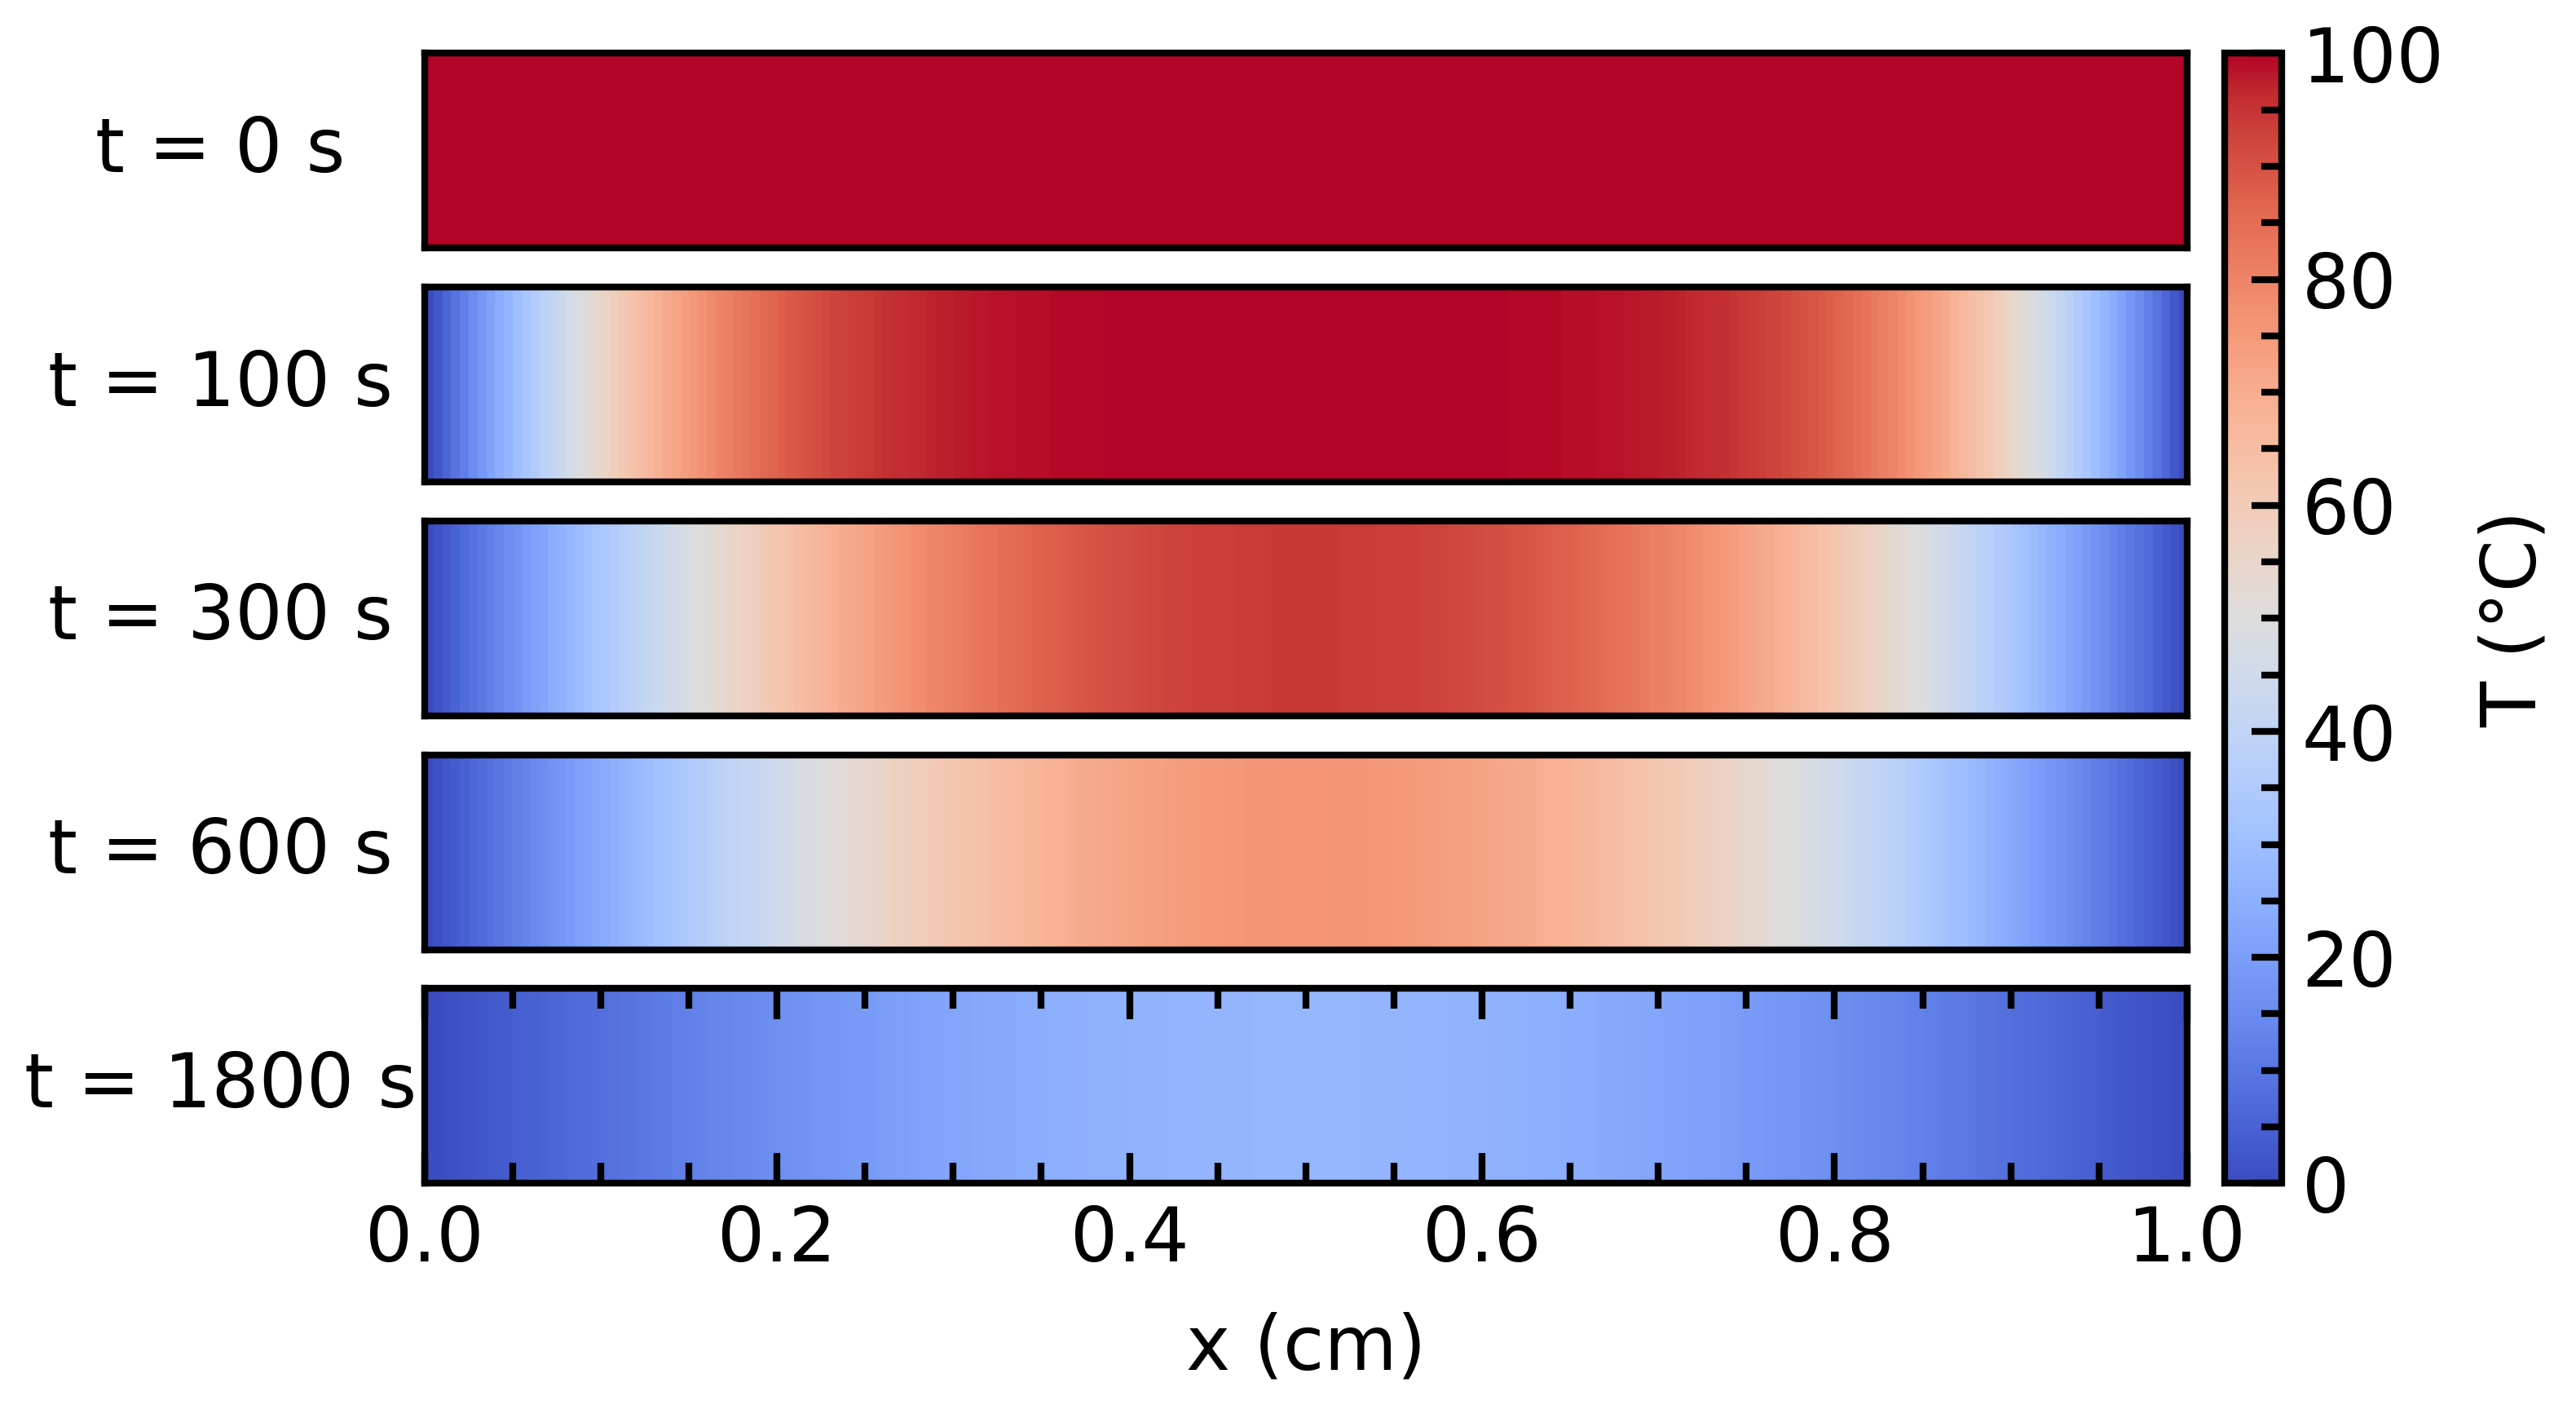
\includegraphics[width=0.85\textwidth]{BTVN7-backward-nhietdo-thanh.png}
    \caption{Ảnh chụp nhanh nhiệt độ thanh tại $t = 0, 100, 300, 600, 1800\,\mathrm{s}$. Thanh nguội dần về phía hai đầu; nhiệt độ tâm giảm theo cấp số nhân với hằng số thời gian $\tau_1 \approx l^2/(\alpha^2 \pi^2) \approx 1172\,\mathrm{s}$.}
    \label{fig:bai1_thanh}
\end{figure}

\subsubsection{Biện luận vật lý}

\begin{itemize}
    \item \textbf{Giai đoạn sớm ($t \le 100\,\mathrm{s}$):} Nhiệt độ biên chỉ truyền được một khoảng $\sqrt{\alpha^2 t} \approx 0.093\,\mathrm{m}$, tức $\sim 9\%$ chiều dài thanh. Lõi thanh vẫn xấp xỉ $100\,^\circ\mathrm{C}$ -- đúng như Hình~\ref{fig:bai1_thanh} hàng 2, vùng đỏ đậm chiếm gần toàn bộ thanh.

    \item \textbf{Giai đoạn chuyển tiếp ($t = 300\!-\!600\,\mathrm{s}$):} Khi $\sqrt{\alpha^2 t}$ tiến gần $l/2$, thông tin từ hai biên ``gặp nhau'' ở giữa.

    \item \textbf{Giai đoạn tiệm cận ($t \approx 1800\,\mathrm{s}$):} Xấp xỉ hàm $\sin(\pi x/l)$ -- mode Fourier cơ bản. Biên độ giảm theo $e^{-t/\tau_1}$; tại $t = 1800\,\mathrm{s}$ ta có $e^{-1800/1172} \approx 0.21$, nên đỉnh xuống còn $\sim 21\%$ giá trị ban đầu.

    \item \textbf{Nghiệm Fourier giải tích:}
    \[
        T(x, t) = \sum_{n=1,3,5,\ldots}^{\infty} \frac{400}{n\pi}\,\sin\!\frac{n\pi x}{l}\,\exp\!\left(-\frac{n^2\pi^2\alpha^2 t}{l^2}\right).
    \]
    Tại thời gian dài, mode $n = 1$ thống trị do decay chậm nhất -- phù hợp quan sát.
\end{itemize}

\subsection{Bài 2: Hai thanh tiếp xúc}

\subsubsection{Tham số hai phương pháp}

\begin{center}
\small
\begin{tabular}{@{}lll@{}}
\toprule
\textbf{Tham số} & \textbf{FTCS} & \textbf{BTCS} \\
\midrule
$N_x$            & 101               & 101 \\
$N_t$            & 15000             & 600 \\
$h$ (m)          & $0.00500$         & $0.00500$ \\
$k$ (s)          & $0.1200$          & $3.0050$ \\
$\eta$           & $0.415$ \checkmark & $10.39$ \emph{(>> 0.5!)} \\
$\beta_1$        & --                & $0.4770$ \\
$\beta_2$        & --                & $0.0459$ \\
\bottomrule
\end{tabular}
\end{center}

Một lần nữa, BTCS dùng $\eta \approx 10.4$, vượt xa giới hạn ổn định của FTCS.

\subsubsection{Số vòng lặp Gauss--Seidel (BTCS)}

\begin{center}
\small
\begin{tabular}{@{}cccccccccccc@{}}
\toprule
Bước $j$   & 50 & 100 & 150 & 200 & 250 & 300 & 350 & 400 & 450 & 500 & 550 \\
\midrule
Số vòng GS & 168 & 162 & 157 & 152 & 146 & 141 & 135 & 130 & 124 & 119 & 113 \\
\bottomrule
\end{tabular}
\end{center}

\textbf{Khác biệt với Bài 1:} Số vòng GS giảm \emph{rõ rệt hơn} theo thời gian (từ 168 xuống 113, giảm $\sim 33\%$, so với Bài 1 chỉ giảm $\sim 7\%$). Lý do: Bài 2 có thời gian đặc trưng ngắn hơn ($\tau_1 \approx 293$ s), nhiệt độ nguội nhanh hơn, điểm xuất phát Gauss--Seidel dần tiến sát nghiệm.

\subsubsection{Phân bố nhiệt độ không--thời gian}

\begin{figure}[H]
    \centering
    \includegraphics[width=0.85\textwidth]{BTVN7-backward-2thanh-3D.png}
    \caption{Bề mặt $T(x, t)$ của Bài 2 (BTCS). Cạnh $t = 0$ là hàm bậc thang: thanh trái $100\,\mathrm{K}$, thanh phải $50\,\mathrm{K}$. Bậc thang được làm mượt tại điểm tiếp xúc trước khi toàn thanh nguội về $0$.}
    \label{fig:bai2_3D}
\end{figure}

\begin{figure}[H]
    \centering
    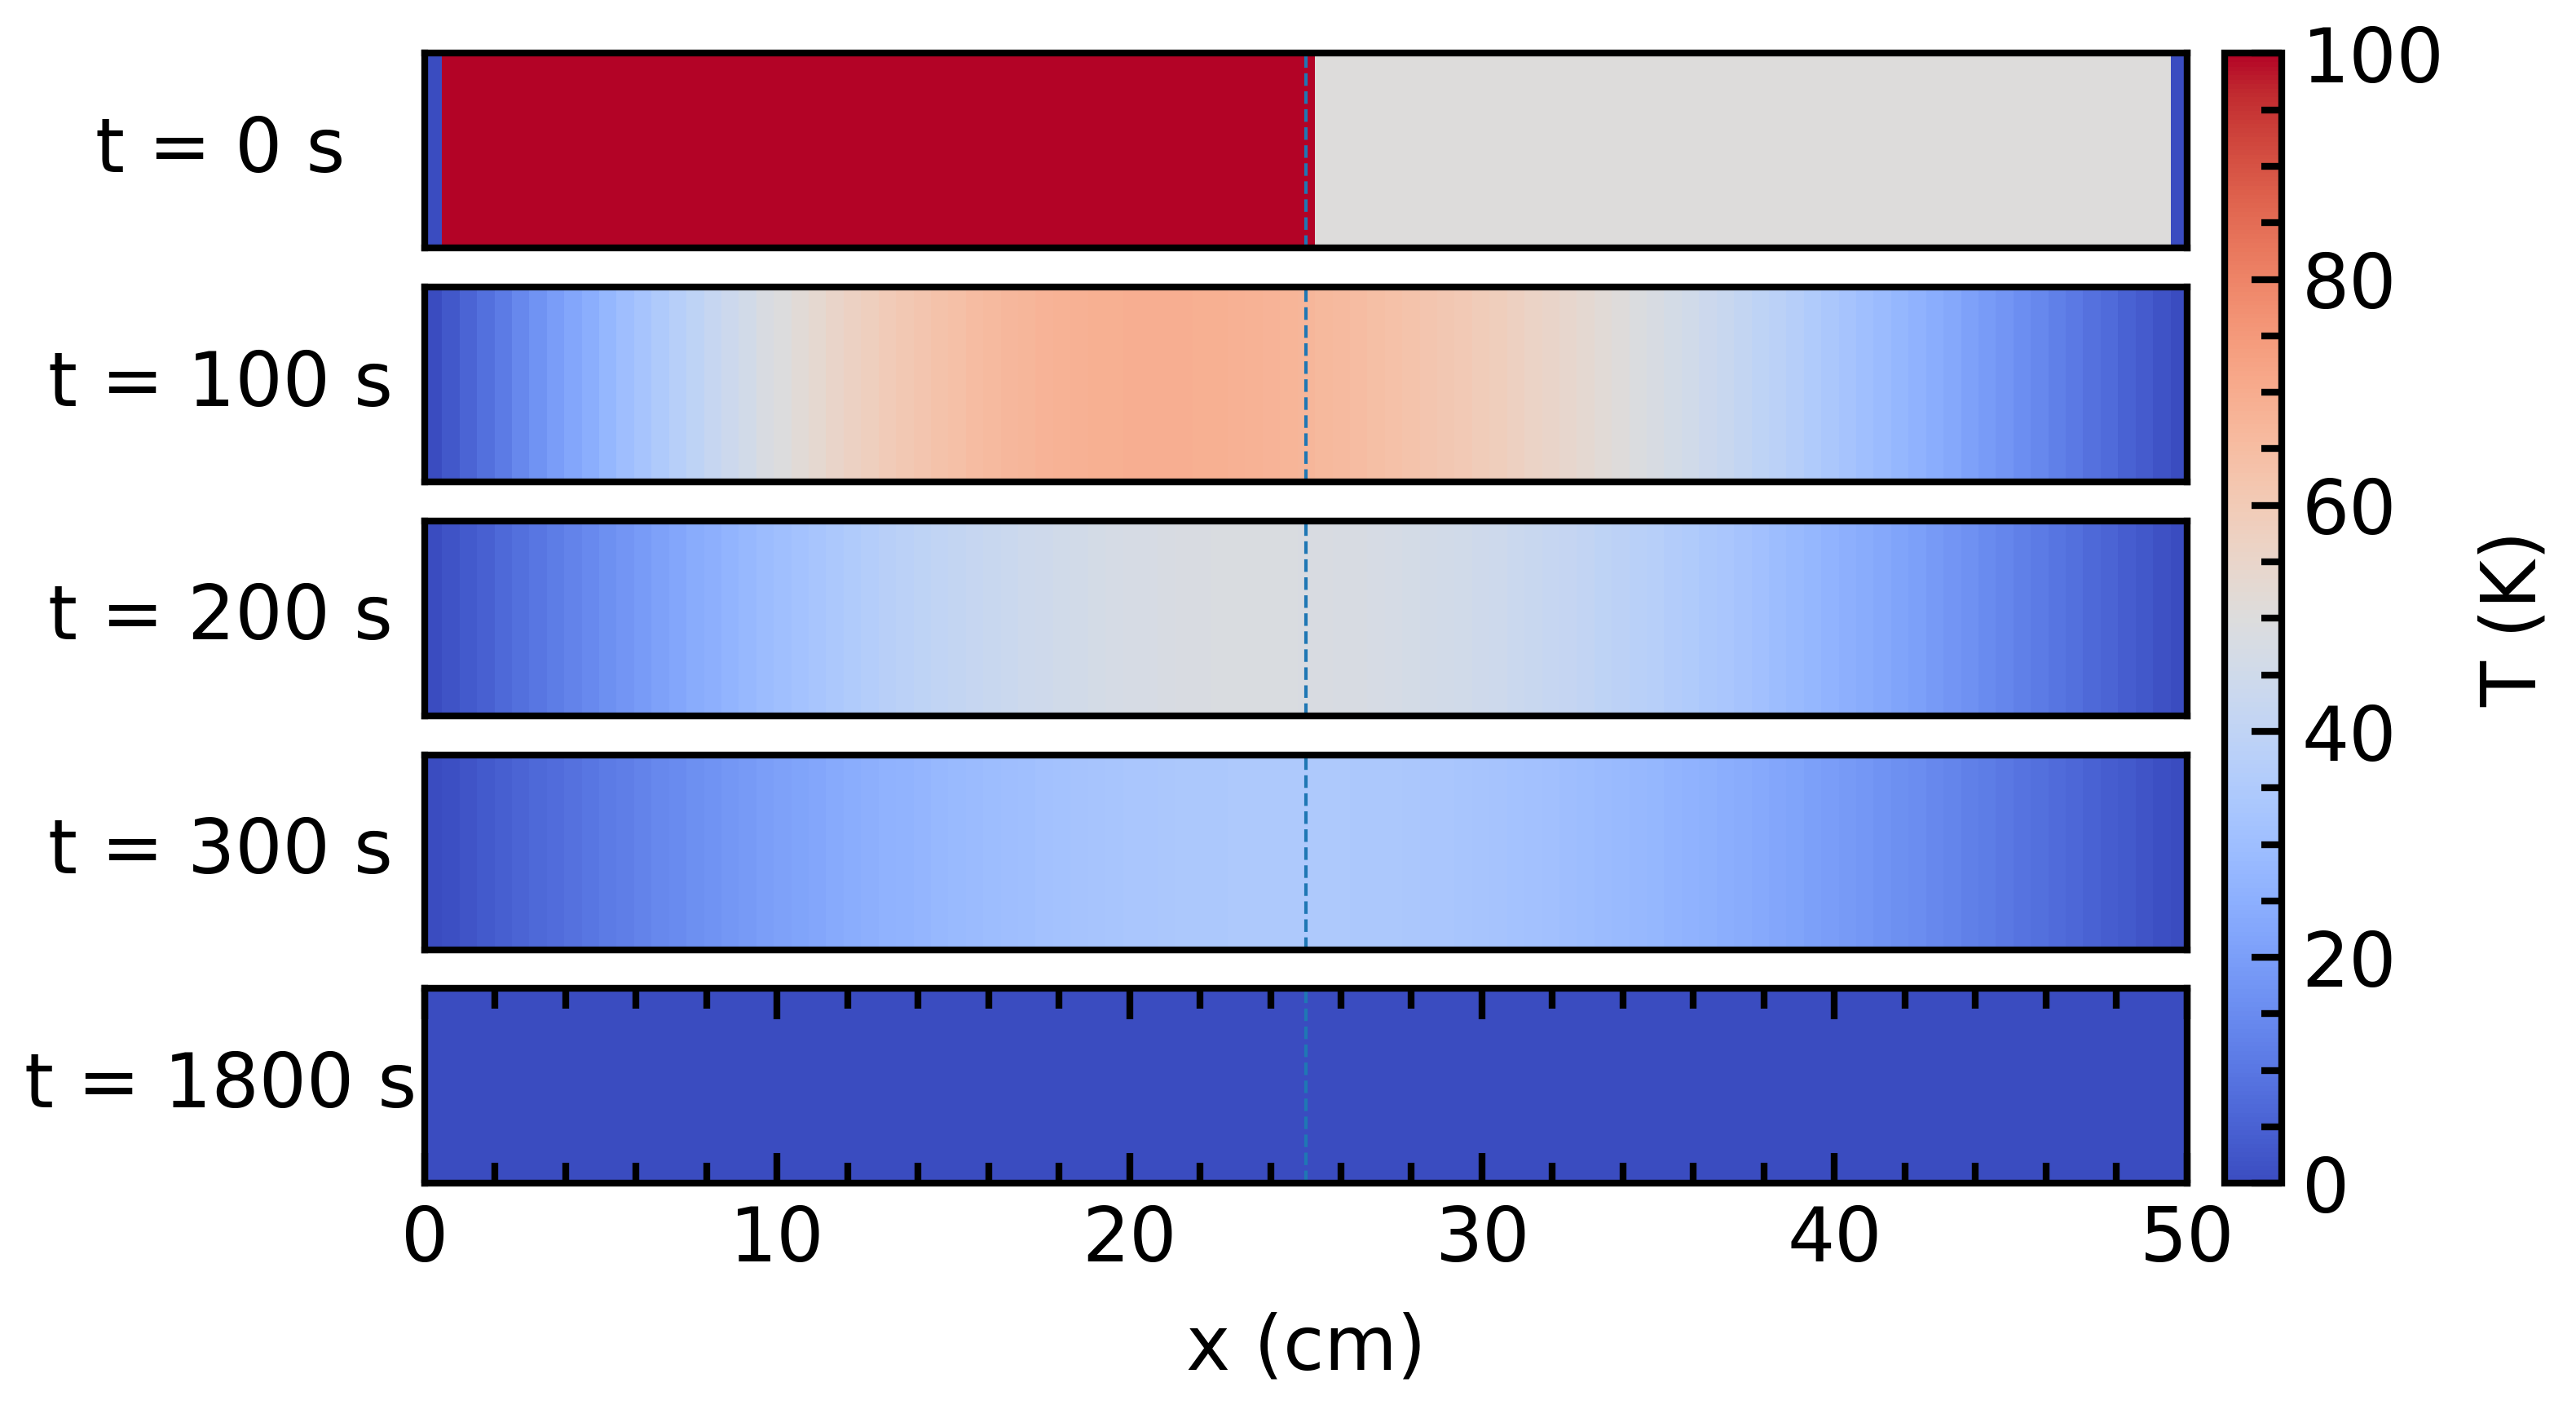
\includegraphics[width=0.85\textwidth]{BTVN7-backward-2thanh-snapshots.png}
    \caption{Ảnh snapshot tại $t = 0, 100, 200, 300, 1800\,\mathrm{s}$. Đường đứt nét $x = 25\,\mathrm{cm}$ đánh dấu điểm tiếp xúc hai thanh. Làm mượt điểm gián đoạn diễn ra trong vài trăm giây đầu.}
    \label{fig:bai2_snap}
\end{figure}

\subsubsection{Biện luận vật lý}

\begin{itemize}
    \item \textbf{Hai thang thời gian khác biệt:}
    \begin{itemize}
        \item \emph{Thang nhanh (làm mượt điểm tiếp xúc):} Khi $t \sim 30\!-\!100\,\mathrm{s}$, sự chênh lệch $100 \to 50\,\mathrm{K}$ tại $x = 0.25\,\mathrm{m}$ được làm mượt, chỉ ảnh hưởng một vùng cỡ $\sqrt{\alpha^2 t}$ quanh điểm tiếp xúc.
        \item \emph{Thang chậm (nguội chung về 0):} Toàn thanh nguội về $0\,\mathrm{K}$ với hằng số thời gian $\tau_1 \approx l_{\text{total}}^2/(\alpha^2 \pi^2) \approx 293\,\mathrm{s}$ -- ngắn hơn $4\times$ so với Bài 1 vì $l$ ngắn $2\times$ (và $\tau \propto l^2$).
    \end{itemize}

    \item \textbf{Ảnh snapshot $t = 100\,\mathrm{s}$:} Vùng điểm tiếp xúc $[0.2, 0.3]\,\mathrm{m}$ đã mượt; hai cao nguyên giữa mỗi thanh còn xấp xỉ $100$ và $50\,\mathrm{K}$. Biên $0\,\mathrm{K}$ đã ảnh hưởng vùng $x \in [0, 0.05]$ và $[0.45, 0.5]$.

    \item \textbf{Ảnh snapshot $t = 300\,\mathrm{s}$:} Không còn phân biệt hai thanh; profile là đường cong trơn liên tục, đỉnh lệch nhẹ về phía thanh trái (do thanh trái ban đầu nóng hơn).

    \item \textbf{Ảnh snapshot $t = 1800\,\mathrm{s}$:} Thanh gần như nguội hết. 
    
\end{itemize}

% =============================================================
\section{Kết luận}
% =============================================================

Bài tập đã thực hiện thành công việc giải phương trình truyền nhiệt 1D bằng hai phương pháp sai phân khác nhau. Các điểm chính rút ra:

\begin{enumerate}
    \item \textbf{Phương pháp FTCS} Phương trình~\eqref{eq:FTCS} đơn giản và rẻ nhất mỗi bước -- chỉ cần ba điểm láng giềng ở bước trước, không cần giải hệ. Đánh đổi là ràng buộc ổn định $\eta \le 1/2$ Phương trình~\eqref{eq:CFL_explicit}, khiến bước thời gian phải nhỏ tỉ lệ với $h^2$.

    \item \textbf{Phương pháp BTCS} Phương trình~\eqref{eq:BTCS_linear} phức tạp hơn ở chỗ phải giải hệ tridiagonal mỗi bước, nhưng đổi lại \emph{ổn định không điều kiện} Phương trình~\eqref{eq:unconditional}. Trong chương trình này, hệ tridiagonal được giải bằng Gauss--Seidel, hội tụ sau $\sim 100\!-\!170$ vòng mỗi bước thời gian (do ma trận chéo trội nghiêm ngặt với $\eta$ lớn).

    \item \textbf{Bài 1 và Bài 2} đều cho kết quả vật lý hợp lý: Bài 1 phân rã thành mode Fourier cơ bản $\sin(\pi x/l)$, Bài 2 làm mượt đoạn điểm tiếp xúc trong thang thời gian nhanh rồi nguội chung về biên trong thang chậm.

\end{enumerate}

\end{document}